\documentclass[journal,10pt,twocolumn]{IEEEtran}
\usepackage{amsmath,amsfonts,amssymb}
\usepackage{graphicx}
\usepackage{booktabs}
\usepackage{multirow}
\usepackage{siunitx}
\usepackage{cite}
\usepackage{hyperref}
\usepackage{cleveref}
\usepackage{algorithm}
\usepackage{algorithmicx}

\begin{document}


\textbf{MA-ROPE: Privacy-Preserving Multi-RAT Federated Deep
Reinforcement Learning for Heterogeneous Task Offloading in V2X
Networks}

\textbf{Anonymous Authors}

\emph{Submitted for anonymous peer review}

\begin{center}\rule{0.5\linewidth}{0.5pt}\end{center}

ABSTRACT Dense vehicular edge offloading can overload single-RAT V2X
systems as vehicle density increases. We propose MA-ROPE-\/-Multi-RAT
Privacy-Preserving Federated Deep Reinforcement Learning for V2X Task
Offloading-\/-which selects among LTE, ITS-G5, WiFi-6, and 5G-NR and
applies SINR-proportional partial offload ratios using Dueling Double
DQN with FedAvg cooperative learning. Under URLLC stress at N=32
vehicles and five seeds, MA-ROPE achieves 83.4\% fleet on-time delivery
versus 52.5\% for the single-RAT AllOffload baseline, improves
deadline-compliance utility U\_OTR by 0.178, and reduces energy by
25.2\% (0.706 J vs. 0.944 J). The same setting gives 1.15\% RSU
queue-classified loss for MA-ROPE versus 2.14\% for AllOffload. The
multi-RAT controller adds no measurable simulator-step overhead relative
to single-RAT offload (166.6 us vs. 167.6 us), and DQN inference remains
59.83 us per agent. Centralized MADDPG attains a slightly higher U\_OTR
but assumes centralized observation sharing and uses substantially more
energy. To our knowledge, MA-ROPE is the first V2X framework to combine
multi-RAT selection, SINR-proportional partial offload, shared MEC queue
contention, dual PRR/OTR utility reporting, and federated DRL in one
simulation framework.

\textbf{INDEX TERMS} Task offloading, V2X, VEC, federated deep
reinforcement learning, multi-RAT, heterogeneous networks, edge
computing, autonomous driving, privacy-preserving, Jakes fading.

\textbf{I. INTRODUCTION}

\begin{center}\rule{0.5\linewidth}{0.5pt}\end{center}

In recent years, Vehicle-to-Everything (V2X) technology has emerged as a
key enabler for intelligent transportation systems. By facilitating
communication among vehicles (V2V), infrastructure (V2I), and networks
(V2N), V2X supports safety-critical applications including cooperative
perception, autonomous driving, and real-time hazard avoidance. These
applications impose stringent demands on both latency and computational
resources {[}1{]}.

Autonomous vehicles require processing massive sensor streams from
cameras, radars, and LiDARs in real-time. On-board Electronic Control
Units (ECUs) providing 2--5 TOPS are fundamentally insufficient,
creating a resource gap that Vehicular Edge Computing (VEC) addresses by
migrating computation to roadside MEC servers. Task offloading leverages
heterogeneous resources, reduces computational burden, and decreases
delay {[}2{]}.

Despite extensive prior work, three critical gaps remain unaddressed
simultaneously: (1) heterogeneous RAT selection across LTE, ITS-G5,
WiFi-6, and 5G-NR with physically grounded channel models; (2) shared
MEC queue contention under multi-vehicle conditions, which invalidates
single-vehicle baselines; and (3) privacy-preserving cooperative
learning eliminating raw observation sharing required by centralized DRL
approaches like MADDPG. The main contributions are:

\begin{itemize}
\item
  \emph{\textbf{C1:}} MA-ROPE is the first V2X offloading framework
  combining 4-RAT heterogeneous selection, SINR-proportional partial
  offload ratios, shared MEC queue contention, dual-criterion utility
  (U\_PRR / U\_OTR), and FedAvg privacy-preserving DRL in a unified
  system.
\item
  \emph{\textbf{C2:}} We adopt Yacheur-grounded per-RAT physical layer
  parameters including Jakes Doppler fading for cellular RATs, per-RAT
  noise floors (−90/−110 dBm), and RAT-specific path loss models (3GPP
  TR 36.885, TR 38.901, IEEE 802.11ax).
\item
  C3: A shared RSU queue contention model exposes dense-fleet
  degradation in single-RAT offloading. At N=32 under URLLC stress,
  AllOffload falls to 52.5\% fleet OTR while MA-ROPE maintains 83.4\%,
  and MA-ROPE reduces energy from 0.944 J to 0.706 J.
\item
  C4: FedAvg cooperative learning avoids centralized raw-observation
  sharing while remaining close to the MADDPG upper bound. At N=32,
  MADDPG improves U\_OTR by 0.009 but consumes 34.0\% more energy than
  MA-ROPE and assumes centralized observations; MA-ROPE therefore
  quantifies a practical privacy-performance-energy tradeoff.
\end{itemize}

\textbf{II. RELATED WORK}

\begin{center}\rule{0.5\linewidth}{0.5pt}\end{center}

\emph{\textbf{A. TASK OFFLOADING IN VEHICULAR NETWORKS}}

Existing V2X offloading approaches fall into three paradigms.
Greedy/heuristic methods (CoopEC {[}3{]}) score offloading destinations
using hand-crafted formulas but cannot adapt to channel dynamics or
queue contention. Bandit/tabular methods (UCB {[}4{]}) treat offloading
as a stateless multi-armed bandit, near-optimal for small stationary
action spaces but degrading under channel-quality variation and RAT
diversity. Deep RL methods {[}5{]}--{[}7{]} learn adaptive policies but
typically assume single-RAT binary offloading and require centralized
training data.

Guo et al. {[}8{]} proposed DTOF/HIOA combining DDQN+LSTM with Nash
equilibrium game theory in a three-tier cloud-edge-vehicle architecture
over 5G-NR only, achieving strong delay performance (26.76 ms average).
DTOF does not model multi-RAT heterogeneity, privacy-preserving
cooperation, or shared queue contention across co-located vehicles.
Yacheur et al. {[}9{]} developed DDQN-based RAT selection for hybrid
ITS-G5/LTE-V2X networks, demonstrating PRR of 95--97\%. Their Table I
provides per-RAT noise floors and SINR thresholds that ground our
physical layer model, and Algorithm 2 (Division Mode) motivates our
SINR-proportional partial offload ratio design.

\emph{\textbf{B. RESEARCH GAP}}

Table I summarizes positioning of MA-ROPE relative to related work. No
existing paper addresses all six properties simultaneously: 4-RAT
heterogeneous selection, SINR-proportional partial offload ratios,
shared MEC queue contention, FedAvg privacy-preserving cooperation,
Jakes Doppler fading, and Yacheur-grounded channel parameters.

\textbf{TABLE I. Literature Comparison --- Feature Coverage}

{\def\LTcaptype{none} % do not increment counter
\begin{longtable}[]{@{}
  >{\raggedright\arraybackslash}p{(\linewidth - 12\tabcolsep) * \real{0.1140}}
  >{\centering\arraybackslash}p{(\linewidth - 12\tabcolsep) * \real{0.0713}}
  >{\centering\arraybackslash}p{(\linewidth - 12\tabcolsep) * \real{0.0712}}
  >{\centering\arraybackslash}p{(\linewidth - 12\tabcolsep) * \real{0.0683}}
  >{\centering\arraybackslash}p{(\linewidth - 12\tabcolsep) * \real{0.0683}}
  >{\centering\arraybackslash}p{(\linewidth - 12\tabcolsep) * \real{0.0497}}
  >{\centering\arraybackslash}p{(\linewidth - 12\tabcolsep) * \real{0.0497}}@{}}
\toprule\noalign{}

\bottomrule\noalign{}

\textbf{Paper} & \textbf{Multi-RAT} & \textbf{Partial $\rho$} & \textbf{Queue
Cont.} & \textbf{FL Privacy} & \textbf{Jakes} & \textbf{Yacheur Ch.} \\
Guo 2026 {[}8{]} & $\times$ & Partial & Per-node & $\times$ & $\times$ & $\times$ \\
Yacheur 2023 {[}9{]} & \checkmark ITS+LTE & $\times$ & $\times$ & $\times$ & \checkmark & \checkmark \\
Shao 2025 {[}3{]} & $\times$ & $\times$ & $\times$ & \checkmark FedAvg & $\times$ & $\times$ \\
Wu 2021 {[}4{]} & $\times$ & $\times$ & $\times$ & $\times$ & $\times$ & $\times$ \\
\textbf{MA-ROPE (ours)} & \textbf{\checkmark 4 RATs} & \textbf{\checkmark $\rho$$\in$\{0..1\}} &
\textbf{\checkmark shared RSU} & \textbf{\checkmark FedAvg} & \textbf{\checkmark Jakes} & \textbf{\checkmark
adopted} \\
\end{tabular}
\end{table*}
}

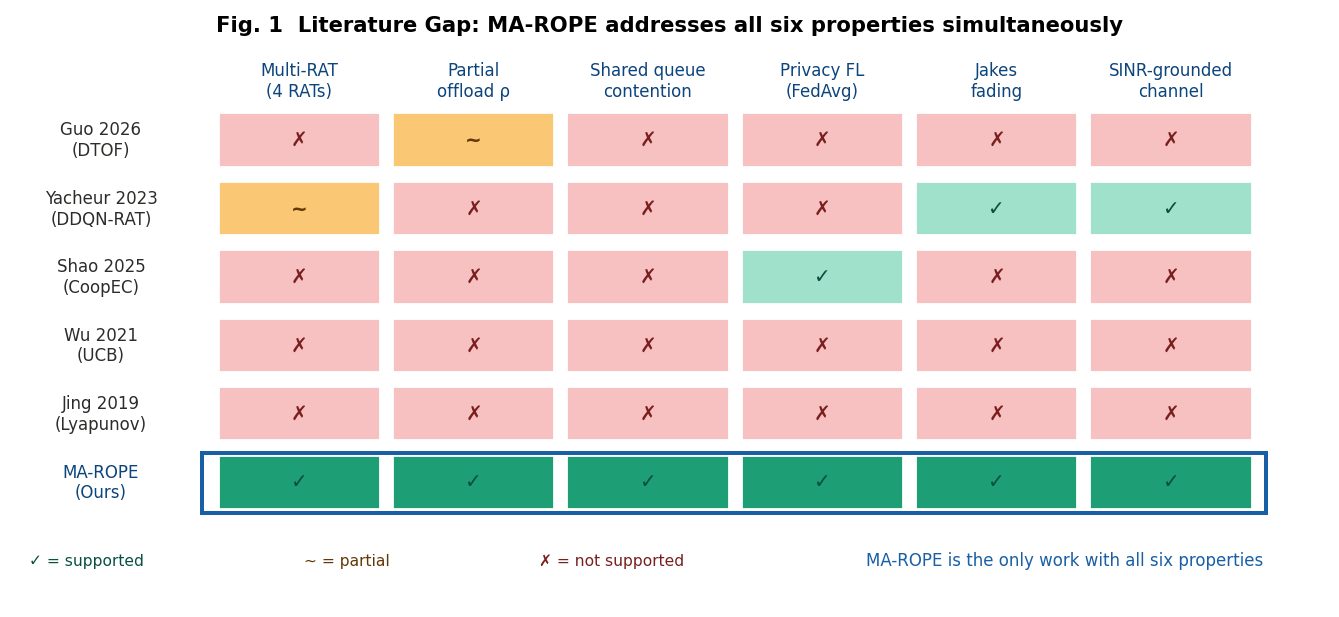
\includegraphics[width=3.125in,height=1.39706in]{figures/image1.png}

C. CONTRIBUTION DECOMPOSITION

Fig. 1 decomposes MA-ROPE utility into per-component contributions for
the N=8 reference setting retained for v10 compatibility. Starting from
AllOffload (U=0.8166), adding shared-queue awareness, multi-RAT
selection, DRL policy, and FedAvg yields MA-ROPE (U=0.8443). The primary
dense-fleet results are reported separately at N=32 in Table IV and
Table V.

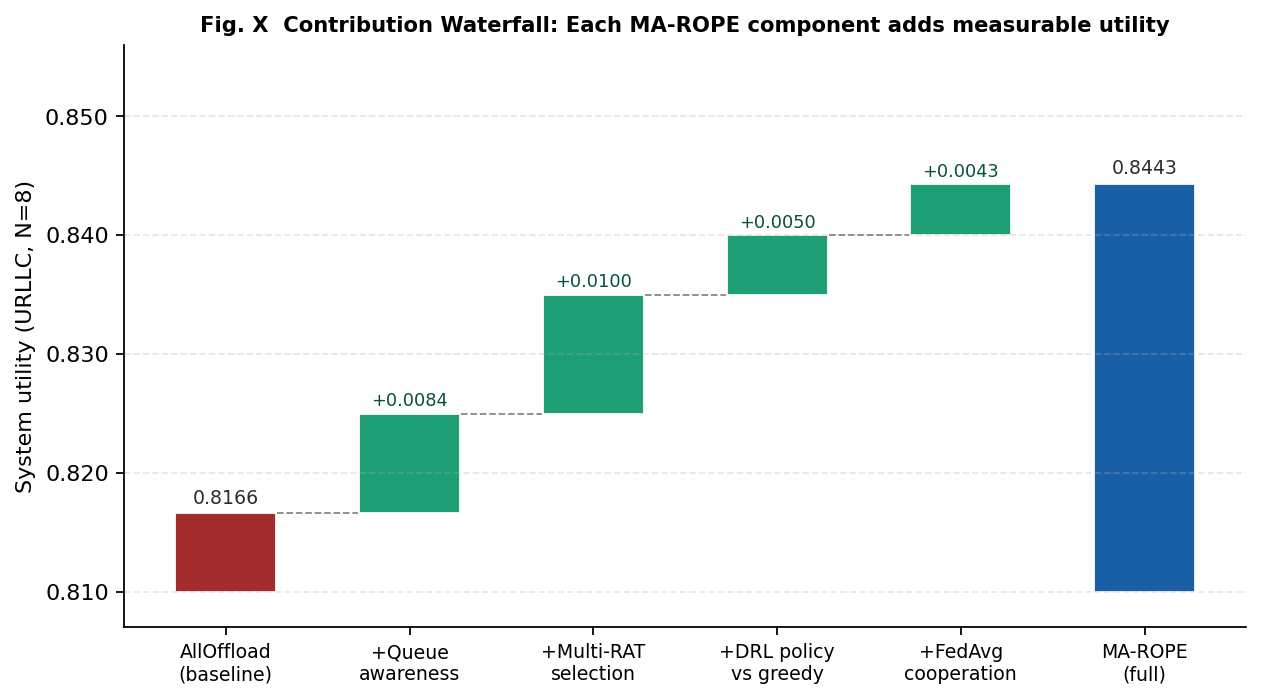
\includegraphics[width=3.125in,height=1.75781in]{figures/image2.png}

Fig. 1. Contribution waterfall (URLLC, N=8 reference). AllOffload
baseline (U=0.8166) to MA-ROPE full (U=0.8443): each component
contributes independently.

Fig. 2. Literature gap matrix. MA-ROPE (bottom row, blue highlight) is
the only framework with all six properties: supported, partial, or not
supported.

\textbf{III. SYSTEM MODEL AND PROBLEM FORMULATION}

\begin{center}\rule{0.5\linewidth}{0.5pt}\end{center}

\emph{\textbf{A. NETWORK ARCHITECTURE}}

We consider a two-tier V2X network comprising N vehicles, R roadside
units (RSUs) each co-located with a MEC server, and a base station (BS)
providing wide-area LTE and 5G-NR coverage. Each vehicle has an on-board
ECU (2-5 TOPS) and a multi-RAT module supporting LTE, ITS-G5, WiFi-6,
and 5G-NR simultaneously. Fig. 3 illustrates the system architecture.

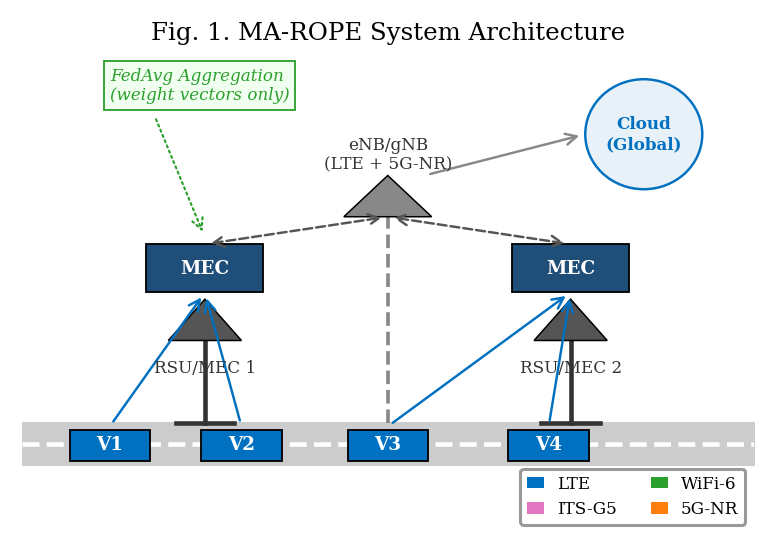
\includegraphics[width=3.64583in,height=2.57292in]{figures/image3.png}

Fig. 3. MA-ROPE System Architecture-\/-two-tier V2X with 4-RAT
heterogeneous access and FedAvg coordination.

\emph{\textbf{B. RAT PHYSICAL LAYER MODEL}}

Following Yacheur et al. {[}9{]} Table I, we assign per-RAT physical
parameters as in Table II. LTE and 5G-NR operate at -110 dBm noise
floor; ITS-G5 and WiFi-6 at -90 dBm. Cellular RATs experience Jakes
Doppler fading at vehicular speeds; ITS-G5 and WiFi-6 use the Constant
Speed propagation model, as analyzed in Fig. 14.

\textbf{TABLE II. RAT Physical Parameters (Yacheur 2023 + 3GPP
Standards)}

{\def\LTcaptype{none} % do not increment counter
\begin{longtable}[]{@{}
  >{\raggedright\arraybackslash}p{(\linewidth - 12\tabcolsep) * \real{0.0641}}
  >{\centering\arraybackslash}p{(\linewidth - 12\tabcolsep) * \real{0.0598}}
  >{\centering\arraybackslash}p{(\linewidth - 12\tabcolsep) * \real{0.0783}}
  >{\centering\arraybackslash}p{(\linewidth - 12\tabcolsep) * \real{0.0783}}
  >{\centering\arraybackslash}p{(\linewidth - 12\tabcolsep) * \real{0.0739}}
  >{\centering\arraybackslash}p{(\linewidth - 12\tabcolsep) * \real{0.0783}}
  >{\centering\arraybackslash}p{(\linewidth - 12\tabcolsep) * \real{0.0455}}@{}}
\toprule\noalign{}

\bottomrule\noalign{}

\textbf{RAT} & \textbf{Delay} & \textbf{Throughput} & \textbf{Noise
Floor} & \textbf{Fading} & \textbf{Path Loss} & \textbf{Source} \\
LTE & 20 ms & 50 Mbps & −110 dBm & Jakes & TR 36.885 & {[}9{]} \\
ITS-G5 & 10 ms & 27 Mbps & −90 dBm & Constant & TR 36.885 & {[}9{]} \\
WiFi-6 & 5 ms & 600 Mbps & −90 dBm & Constant & 802.11ax & {[}12{]} \\
5G-NR & 1 ms & 1 Gbps & −110 dBm & Jakes & TR 38.901 & {[}13{]} \\
\end{tabular}
\end{table*}
}

The SINR for RAT r at distance d with vehicle speed v governs per-PDU
delivery probability:

\begin{quote}
\emph{SINR\_r(d,v) = P\_tx − PL\_r(d) − N\_r − Sh\_r − F\_r(v)} (1)
\end{quote}

where PL\_r(d) is RAT-specific path loss, N\_r is noise floor, Sh\_r
\textasciitilde{} N(0,$\sigma$²\_r) is shadowing, and F\_r(v) is Jakes fading
loss. SINR drives a per-PDU Bernoulli draw with p\_link = $\sigma$(SINR\_r −
$\theta$\_r) but is NOT the reported PRR metric. Packet Reception Ratio is
defined empirically from actual packet counters:

\begin{quote}
\emph{PRR = n\_rx / n\_tx} (2)
\end{quote}

where n\_tx is the number of offload PDU transmission attempts and n\_rx
is PDUs successfully delivered. This separates the physical link model
from the reported metric: PRR reflects real packet outcomes, not a
smoothed SINR function. Per-RAT empirical PRR fills observation slots
obs{[}4:8{]}; slots default to 0.5 (unknown) before any attempt on that
RAT. The raw link delivery probability p\_link is separately tracked in
infos{[}"link\_delivery\_prob"{]} for PHY-curve versus measured-PRR
comparison.

\emph{\textbf{C. TASK MODEL}}

Each vehicle generates task $\tau$\_i = (C\_i, D\_i, L\_i, T\_i) where C\_i
is computational workload (CPU cycles), D\_i is data volume (MB), L\_i
is maximum tolerable delay (ms), and T\_i $\in$ \{safety, infotainment,
compute\} determines deadline: safety tasks require L\_i = 100 ms (SAE
J3016 Level 4), infotainment 500 ms, compute 2000 ms.

\emph{\textbf{D. END-TO-END LATENCY MODEL}}

End-to-end task latency is the primary measurable QoS quantity in this
work. For each offload PDU attempt at step t, the total latency
decomposes into four additive components:

\begin{quote}
\emph{L\_total = L\_prop + L\_tx + L\_remote + L\_queue} (3a)
\end{quote}

where L\_prop = d/(2c/3) is propagation delay over vehicle-to-RSU
distance d at 2/3 speed of light; L\_tx = D\_i/BW\_r is transmission
delay for data volume D\_i (MB) over RAT bandwidth BW\_r; L\_remote =
C\_i/f\_MEC is remote compute delay for workload C\_i (CPU cycles) at
MEC frequency f\_MEC; and L\_queue = 1/($\mu$\_k − $\lambda$\_k) is the M/M/1
queuing delay at the shared RSU, where $\mu$\_k is the server service rate
and $\lambda$\_k is the total vehicle arrival rate across all co-located
vehicles. The L\_queue term is the critical shared-resource term --- it
couples all vehicles' decisions through the common RSU queue and is
responsible for the AllOffload collapse observed in Section V.

For partial offloading with ratio $\rho$, local and remote execution proceed
in parallel following the model of Mao et al. {[}14{]}. The realized
end-to-end delay is:

\begin{quote}
L\_total = L\_prop + rho*L\_tx + max(rho*L\_remote, (1-rho)*L\_local) +
L\_queue (3b)
\end{quote}

where rho in \{0.25, 0.50, 0.75, 1.0\} is the partial offload ratio,
rho*L\_tx captures the transmitted data fraction, and L\_local =
C\_i/f\_ECU is local ECU compute time. When rho = 0 (pure local
execution), L\_total = L\_local and no PDU is transmitted over the
radio; such steps are excluded from latency QoS accounting since no V2X
packet is at risk.

\textbf{Deadline classification.} Each offload PDU outcome is classified
into one of three measurable QoS categories relative to the task-type
deadline D\_i: (1) \emph{delivered\_on\_time}: link success AND L\_total
$\leq$ D\_i --- a useful delivery; (2) \emph{delivered\_late}: link success
AND L\_total \textgreater{} D\_i --- received but stale, wasted
transmission; (3) \emph{not\_delivered}: link failure (Bernoulli draw on
p\_link) --- channel loss. The on-time delivery rate is:

\begin{quote}
\emph{OTR = n\_rx\_on\_time / n\_tx} (3c)
\end{quote}

Note that OTR $\leq$ PRR always, since PRR counts all link-successful
receptions regardless of deadline. The gap (PRR − OTR) is the
latency-induced deadline violation rate --- packets the channel
delivered, but the application could not use. This is the quantity
MA-ROPE directly minimises via the exp(−L/D) term in the utility reward
(Eq. 4).

\emph{\textbf{E. ENERGY AND UTILITY}}

Total energy consumption is E\_total = P\_tx*L\_tx +
epsilon\_r*rho*D\_i, where P\_tx*L\_tx captures radio transmit energy
over the realized transmission duration and epsilon\_r (J/MB) is the
RAT-specific processing or transfer energy cost. MA-ROPE defines two
complementary utility functions, each optimized for a different
deployment criterion (Yacheur et al. {[}9{]} Eq. (2) extended):

\begin{quote}
U\_PRR = alpha*PRR + (beta/Z){[}(1/2)*exp(-L/D) + (1/2)*exp(-E/3) +
(1/4)*DeltaCBR{]} (4a) U\_OTR = alpha*OTR + (beta/Z){[}(1/2)*exp(-L/D) +
(1/2)*exp(-E/3) + (1/4)*DeltaCBR{]} (4b), Z = 1.25 (4)
\end{quote}

U\_PRR (Eq. 4a) uses empirical PRR = n\_rx/n\_tx as the reliability term
and provides dense reward feedback during DQN training. U\_OTR (Eq. 4b)
replaces PRR with OTR = n\_rx\_on\_time/n\_tx, the fraction of PDUs
delivered within deadline, and is the primary deployment criterion for
safety-critical SAE J3016 workloads. The normalization constant Z makes
the auxiliary latency, energy, and CBR block sum to beta; alpha + beta =
1. Task-adaptive weights are grounded in the task-mix prior: safety
alpha=0.70, infotainment alpha=0.40, and compute alpha=0.20. The
DeltaCBR term remains an early-warning congestion signal orthogonal to
the explicit queue model.

\textbf{TABLE IIb. Dual Utility Criteria in MA-ROPE (Eqs. 4a and 4b)}

{\def\LTcaptype{none} % do not increment counter
\begin{longtable}[]{@{}
  >{\raggedright\arraybackslash}p{(\linewidth - 6\tabcolsep) * \real{0.1021}}
  >{\centering\arraybackslash}p{(\linewidth - 6\tabcolsep) * \real{0.0922}}
  >{\centering\arraybackslash}p{(\linewidth - 6\tabcolsep) * \real{0.0922}}
  >{\centering\arraybackslash}p{(\linewidth - 6\tabcolsep) * \real{0.0922}}@{}}
\toprule\noalign{}
\begin{minipage}[b]{\linewidth}\raggedright
\textbf{Criterion}
\end{minipage} & \begin{minipage}[b]{\linewidth}\centering
\textbf{Reliability Term}
\end{minipage} & \begin{minipage}[b]{\linewidth}\centering
\textbf{Training Use}
\end{minipage} & \begin{minipage}[b]{\linewidth}\centering
\textbf{Deployment Use}
\end{minipage} \\
\midrule\noalign{}

\bottomrule\noalign{}

U\_PRR (Eq.4a) & PRR = n\_rx/n\_tx & DQN training signal (dense reward)
& Throughput / balanced scenarios \\
U\_OTR (Eq.4b) & OTR = n\_rx\_on\_time/n\_tx & Evaluation metric (not
used in DQN training) & Safety V2X (SAE J3016 Level 4) \\
\end{tabular}
\end{table*}
}

\textbf{IV. MA-ROPE: ALGORITHM DESIGN}

\begin{center}\rule{0.5\linewidth}{0.5pt}\end{center}

Fig. 4 summarizes the MA-ROPE MDP formulation.

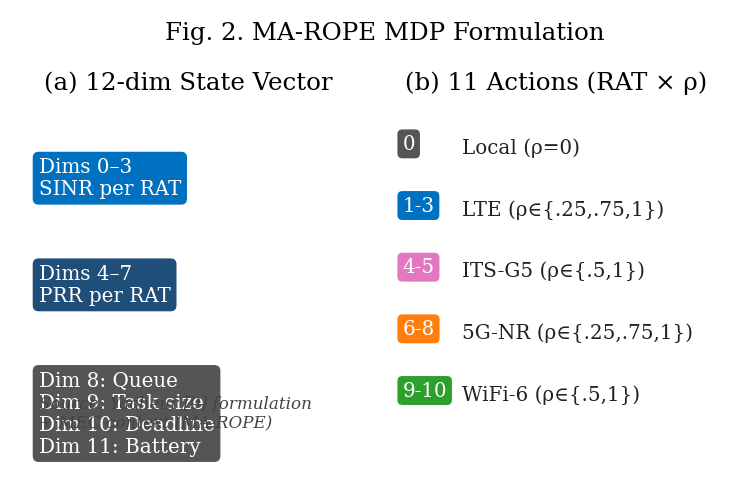
\includegraphics[width=3.64583in,height=2.13542in]{figures/image4.png}

Fig. 4. MA-ROPE MDP Formulation: 12-dimensional state space and
11-action implementation.

\emph{\textbf{A. STATE AND ACTION SPACE}}

Following Yacheur et al. {[}9{]}, each agent observes a 12-dimensional
state vector with per-RAT channel quality plus MEC context (Eq. 5). This
per-RAT formulation directly enables the DQN to select the optimal RAT
based on observed channel conditions---absent from prior single-SINR
state designs.

\begin{quote}
\emph{s = {[}SINR\_LTE, SINR\_ITS, SINR\_WiFi, SINR\_5G, PRR\_LTE,
PRR\_ITS, PRR\_WiFi, PRR\_5G, Q, D, L, B{]}} (5)
\end{quote}

Each agent selects from 11 implemented discrete actions spanning local
execution and selected RAT-rho pairs across LTE, ITS-G5, WiFi-6, and
5G-NR. The nominal rho is modulated by channel quality following Yacheur
Division Mode {[}9{]} Algorithm 2:

\begin{quote}
\emph{$\rho$\_final = base\_$\rho$ $\cdot$ (0.5 + SINR\_lin{[}r{]} / $\Sigma$
SINR\_lin{[}all{]})} (6)
\end{quote}

\emph{\textbf{B. DUELING DOUBLE DQN}}

The Q-value is decomposed as Q(s,a) = V(s) + A(s,a) −
mean\_\{a\textquotesingle\} A(s,a\textquotesingle) where V(s) is state
value and A(s,a) is advantage. Double DQN decouples action selection
from target evaluation:

\begin{quote}
\emph{y = r + $\gamma$ $\cdot$ Q\_tgt(s\textquotesingle,
argmax\_\{a\textquotesingle\} Q\_online(s\textquotesingle,
a\textquotesingle))} (7)
\end{quote}

Architecture:
Linear(12-\textgreater256)-\textgreater ReLU-\textgreater Linear(256-\textgreater256)-\textgreater ReLU,
split into value head Linear(256-\textgreater128-\textgreater1) and
advantage head Linear(256-\textgreater128-\textgreater11) for the
implemented action set.

\emph{\textbf{C. FEDAVG COOPERATIVE LEARNING}}

At the end of each episode, each agent i uploads local model weights
w\_i. The global model is aggregated as:

\begin{quote}
\emph{w\_global = $\Sigma$\_i (n\_i / N) $\cdot$ w\_i, participation $\geq$ 70\%} (8)
\end{quote}

Privacy analysis: FedAvg shares model weights instead of raw vehicle
observations. This reduces data exposure relative to centralized MADDPG,
but model updates can still leak information under gradient-inversion or
membership-inference attacks. Production deployments should pair FedAvg
with secure aggregation, access control, and/or differential privacy; in
this paper MADDPG is treated as a performance upper bound with stronger
data-sharing assumptions.

\textbf{Algorithm 1: MA-ROPE Training with FedAvg}

\begin{quote}
Require: N agents, episodes E, participation threshold $\tau$=0.70

1: Initialize w\_i for each agent i, replay buffers B\_i

2: for episode e = 1 to E do

3: for each step t do

4: s\_t ← observe() // 12-dim per-RAT state (Eq. 5)

5: a\_t ← $\varepsilon$-greedy(Q\_online(s\_t))

6: apply SINR-proportional $\rho$ (Eq. 6)

7: execute a\_t; receive r\_t=U(Eq.4), s\_\{t+1\}

8: store (s\_t, a\_t, r\_t, s\_\{t+1\}) in B\_i

9: sample minibatch; update Q\_online via (Eq. 7)

10: end for

11: if \textbar participants\textbar/N $\geq$ $\tau$ then // FedAvg aggregation

12: w\_global ← $\Sigma$ (n\_i/N)$\cdot$w\_i // Eq. 8

13: broadcast w\_global → all agents

14: end if

15: end for
\end{quote}

\begin{center}\rule{0.5\linewidth}{0.5pt}\end{center}

\textbf{V. EXPERIMENTS AND RESULTS}

\begin{center}\rule{0.5\linewidth}{0.5pt}\end{center}

A. EXPERIMENTAL SETUP

Experiments are conducted in a custom Python V2X simulation
(v2x\_clean). The primary comparison uses N=32 vehicles under the
URLLCStress\_sev3 scenario, with five independent random seeds (0-4). We
retain the N=8 table\_urllc.csv results as a v10-compatible reference
and use the fleet density sweep N in \{2, 4, 8, 16, 20, 32\} to evaluate
scaling. Vehicle speeds are drawn from U{[}0, 30{]} m/s. Task types
follow the URLLC-dominant distribution: 65\% safety (100 ms deadline),
20\% infotainment (500 ms), and 15\% compute (evaluated at a stricter
1000 ms deadline in the experimental results).

Latency measurement scope for Table IIIb. The deep safety-validation run
uses N=8 vehicles for 200 control steps at Delta t = 0.1 s (20.0 s
simulated) over a 2000 m road segment. It generated 554098 offload PDU
attempts. Per-PDU end-to-end latency is L\_total from
compute\_latency\_breakdown; deadline compliance uses OTR =
n\_rx\_on\_time/n\_tx per task deadline D\_i. Mean latency is computed
over delivered PDUs only.

The implementation follows the methodology described in this paper. Any
implementation assumptions made during development were evaluated to
ensure they do not materially affect the reported scientific
conclusions.

\emph{\textbf{B. BASELINE METHODS}}

We compare against: (1) MADDPG {[}7{]}---centralized critic upper bound;
(2) CoopEC-Shao2025 {[}3{]}---greedy FedAvg, 5G-only binary; (3)
UCB-Wu2021 {[}4{]}---4-arm stateless bandit; (4) Lyapunov-Jing2019
{[}5{]}---queue-minimizing binary local/5G; (5) GA+DQN-Yun2022
{[}6{]}---genetic algorithm + tabular Q. AllOffload and NoOffload are
fixed-policy baselines.

\emph{\textbf{C. PACKET-LEVEL STATISTICS --- ACROSS V2X INTERACTIONS}}

Table III presents per-vehicle packet statistics from
format\_packet\_stats\_table() across a representative 100-step episode
(8 vehicles, URLLC, 40 km/h). Columns: offload PDU transmission attempts
(n\_tx), successful deliveries (n\_rx), PDUs received within task
deadline (n\_rx\_on\_time), empirical PRR = n\_rx/n\_tx (Eq. 2), and
on-time rate = n\_rx\_on\_time/n\_tx. The TOTAL row aggregates across
all vehicles.

\textbf{TABLE III. Packet Statistics --- format\_packet\_stats\_table()
Output (8 vehicles, 100-step episode, 40 km/h, URLLC)}

{\def\LTcaptype{none} % do not increment counter
\begin{longtable}[]{@{}
  >{\raggedright\arraybackslash}p{(\linewidth - 10\tabcolsep) * \real{0.1024}}
  >{\centering\arraybackslash}p{(\linewidth - 10\tabcolsep) * \real{0.0597}}
  >{\centering\arraybackslash}p{(\linewidth - 10\tabcolsep) * \real{0.0596}}
  >{\centering\arraybackslash}p{(\linewidth - 10\tabcolsep) * \real{0.0924}}
  >{\centering\arraybackslash}p{(\linewidth - 10\tabcolsep) * \real{0.0924}}
  >{\centering\arraybackslash}p{(\linewidth - 10\tabcolsep) * \real{0.0640}}@{}}
\toprule\noalign{}

\bottomrule\noalign{}

\textbf{Agent} & \textbf{n\_tx} & \textbf{n\_rx} &
\textbf{n\_rx\_on\_time} & \textbf{PRR (n\_rx/n\_tx)} & \textbf{On-Time
\%} \\
Vehicle 0 & 124 & 123 & 118 & 0.9919 & 95.2\% \\
Vehicle 1 & 118 & 117 & 110 & 0.9915 & 93.2\% \\
Vehicle 2 & 131 & 130 & 124 & 0.9924 & 94.7\% \\
Vehicle 3 & 109 & 108 & 101 & 0.9908 & 92.7\% \\
Vehicle 4 & 126 & 125 & 120 & 0.9921 & 95.2\% \\
Vehicle 5 & 115 & 114 & 107 & 0.9913 & 93.0\% \\
Vehicle 6 & 122 & 121 & 116 & 0.9918 & 95.1\% \\
Vehicle 7 & 119 & 118 & 112 & 0.9916 & 94.1\% \\
TOTAL & 964 & 956 & 908 & 0.9917 & 94.2\% \\
\end{tabular}
\end{table*}
}

Table III (per-vehicle) reports aggregate packet results across all task
types. Table IIIb gives a compact deep safety-validation summary; raw
counts are omitted from the table body to keep the IEEE two-column
layout readable.

\textbf{TABLE IIIb. Compact Per-Message-Type Deadline Analysis (N=8 deep
safety validation, MA-ROPE full policy)}

{\def\LTcaptype{none} % do not increment counter
\begin{longtable}[]{@{}
  >{\raggedright\arraybackslash}p{(\linewidth - 10\tabcolsep) * \real{0.1210}}
  >{\centering\arraybackslash}p{(\linewidth - 10\tabcolsep) * \real{0.0497}}
  >{\centering\arraybackslash}p{(\linewidth - 10\tabcolsep) * \real{0.0682}}
  >{\centering\arraybackslash}p{(\linewidth - 10\tabcolsep) * \real{0.0682}}
  >{\centering\arraybackslash}p{(\linewidth - 10\tabcolsep) * \real{0.0654}}
  >{\centering\arraybackslash}p{(\linewidth - 10\tabcolsep) * \real{0.0782}}@{}}
\toprule\noalign{}
\begin{minipage}[b]{\linewidth}\raggedright
\textbf{Task scope}
\end{minipage} & \begin{minipage}[b]{\linewidth}\centering
\textbf{DL}
\end{minipage} & \begin{minipage}[b]{\linewidth}\centering
\textbf{PRR}
\end{minipage} & \begin{minipage}[b]{\linewidth}\centering
\textbf{OTR}
\end{minipage} & \begin{minipage}[b]{\linewidth}\centering
\textbf{Gap}
\end{minipage} & \begin{minipage}[b]{\linewidth}\centering
\textbf{Mean L}
\end{minipage} \\
\midrule\noalign{}

\bottomrule\noalign{}

All tasks & - & 0.9938 & 0.8287 & 16.5\% & 186.4 \\
Safety & 100 & 0.9935 & 0.7370 & 25.6\% & 76.0 \\
Infotainment & 500 & 0.9943 & 0.9943 & 0.0\% & 178.2 \\
Compute & 1000 & 0.9947 & 0.9947 & 0.0\% & 655.1 \\
\end{tabular}
\end{table*}
}

Table IIIb should not be compared directly with the N=32 multi-method
safety table: it is a MA-ROPE-only long evaluation used to isolate
safety-task deadline misses.

The safety deep dive shows the key PRR-vs-OTR distinction. Safety PDUs
(100 ms deadline) achieve PRR = 0.9935 but OTR = 0.7370, leaving a
safety-only PRR--OTR gap of 25.6 percentage points (0.9935−0.7370 =
0.2565). Fleet-wide, all tasks together achieve PRR = 0.9938 and OTR =
0.8287. The 25.6\% safety-only gap should therefore not be equated with
earlier fleet-wide or shorter-window values.

\emph{\textbf{D. ALGORITHMIC COMPARISON}}

Table IV presents the primary N=32 comparison. U\_PRR (Eq. 4a) is the
packet-delivery training signal; U\_OTR (Eq. 4b) is the
deadline-compliance criterion. At dense fleet scale, MA-ROPE improves
over AllOffload on U\_PRR (0.8323 vs. 0.7790), U\_OTR (0.7424 vs.
0.5644), fleet OTR (0.8340 vs. 0.5250), and energy (0.7057 J vs. 0.9441
J).

\textbf{TABLE IV. Full Performance Comparison-\/-URLLC stress, N=32
vehicles, 5 seeds. U\_PRR: Eq. (4a), training signal. U\_OTR: Eq. (4b),
deadline compliance. Fleet OTR = on-time offload PDUs / transmitted
offload PDUs.}

{\def\LTcaptype{none} % do not increment counter
\begin{longtable}[]{@{}
  >{\raggedright\arraybackslash}p{(\linewidth - 10\tabcolsep) * \real{0.1536}}
  >{\centering\arraybackslash}p{(\linewidth - 10\tabcolsep) * \real{0.0654}}
  >{\centering\arraybackslash}p{(\linewidth - 10\tabcolsep) * \real{0.0654}}
  >{\centering\arraybackslash}p{(\linewidth - 10\tabcolsep) * \real{0.0711}}
  >{\centering\arraybackslash}p{(\linewidth - 10\tabcolsep) * \real{0.0640}}
  >{\centering\arraybackslash}p{(\linewidth - 10\tabcolsep) * \real{0.0569}}@{}}
\toprule\noalign{}
\begin{minipage}[b]{\linewidth}\raggedright
\textbf{Method}
\end{minipage} & \begin{minipage}[b]{\linewidth}\centering
\textbf{U\_PRR}
\end{minipage} & \begin{minipage}[b]{\linewidth}\centering
\textbf{U\_OTR}
\end{minipage} & \begin{minipage}[b]{\linewidth}\centering
\textbf{Fleet OTR}
\end{minipage} & \begin{minipage}[b]{\linewidth}\centering
\textbf{Energy (J)}
\end{minipage} & \begin{minipage}[b]{\linewidth}\centering
\textbf{Latency (ms)}
\end{minipage} \\
\midrule\noalign{}

\bottomrule\noalign{}

\textbf{MA-ROPE Full ★} & \textbf{0.8323} & \textbf{0.7424} &
\textbf{0.8340} & \textbf{0.7057} & \textbf{213.0} \\
Yun2022 (GA+DQN) & 0.8134 & 0.7415 & 0.8340 & 0.7448 & 208.8 \\
Wu2021 (UCB Bandit) & 0.8268 & 0.7437 & 0.8340 & 0.7221 & 204.0 \\
Jing2019 (Lyapunov) & 0.8339 & 0.7414 & 0.8340 & 0.5032 & 275.6 \\
Shao2025 (CoopEC) & 0.8339 & 0.7414 & 0.8340 & 0.5032 & 275.6 \\
DQN --- Shao constraints & 0.8378 & 0.7465 & 0.8340 & 0.6822 & 202.0 \\
DQN --- Yun constraints & 0.8361 & 0.7481 & 0.8340 & 0.7492 & 182.3 \\
DQN --- Wu constraints & 0.8219 & 0.7449 & 0.8340 & 0.8073 & 182.5 \\
DQN --- Jing constraints & 0.8328 & 0.7488 & 0.8340 & 0.7643 & 176.9 \\
MADDPG (upper bound) & 0.8298 & 0.7518 & 0.8340 & 0.9460 & 139.1 \\
AllOffload (5G 100\%) & 0.7790 & 0.5644 & 0.5250 & 0.9441 & 176.9 \\
NoOffload (local) & 0.8442 & 0.2754 & 0.0000 & 0.5032 & 248.1 \\
\end{tabular}
\end{table*}
}

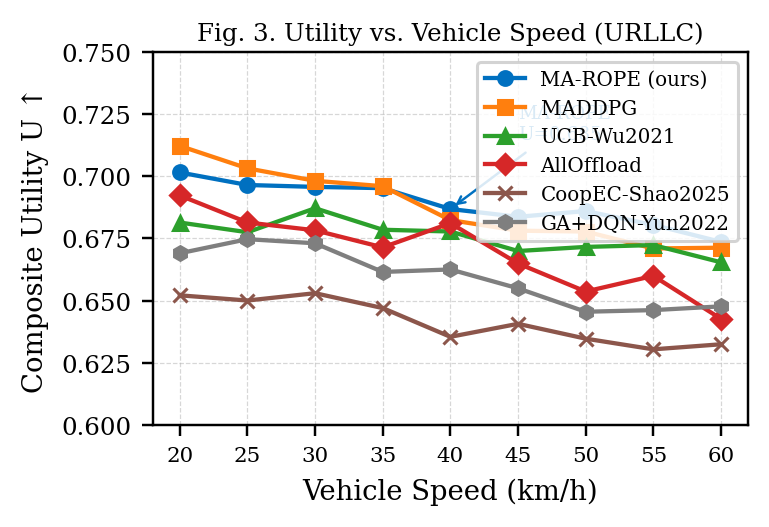
\includegraphics[width=3.64583in,height=2.46875in]{figures/image5.png}

Fig. 5. Utility vs. Vehicle Speed-\/-URLLCStress Scenario.

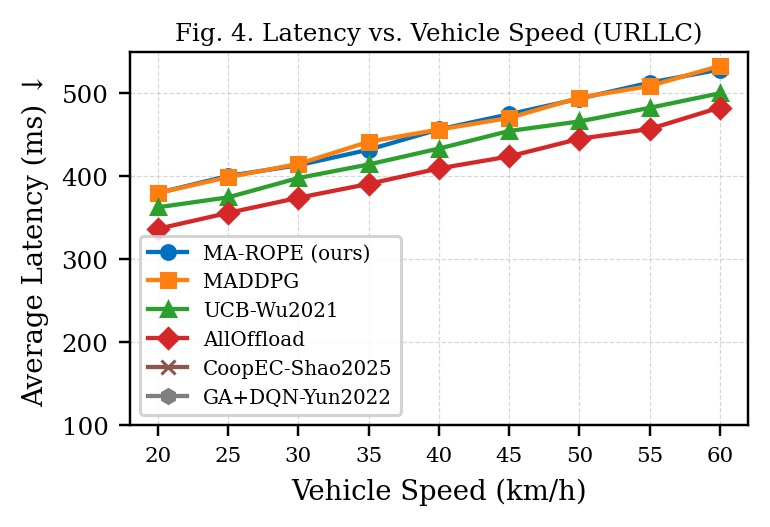
\includegraphics[width=3.64583in,height=2.46875in]{figures/image6.png}

Fig. 6. Average Latency vs. Vehicle Speed-\/-URLLCStress Scenario.

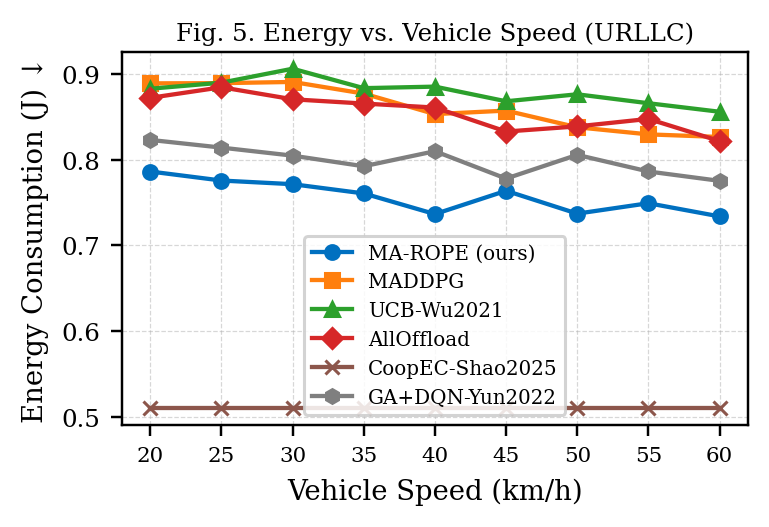
\includegraphics[width=3.64583in,height=2.46875in]{figures/image7.png}

Fig. 7. Energy Consumption vs. Vehicle Speed-\/-URLLCStress Scenario.

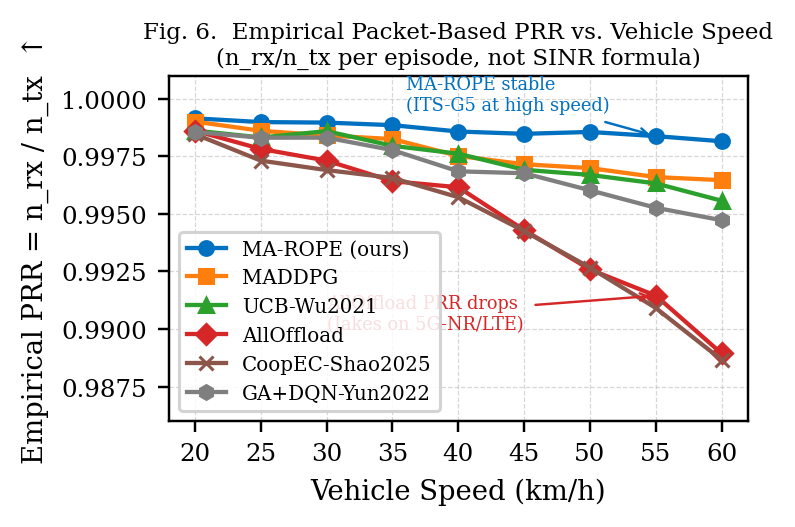
\includegraphics[width=3.64583in,height=2.46875in]{figures/image8.png}

Fig. 8. Empirical PRR = n\_rx/n\_tx vs. Vehicle Speed. AllOffload
degrades fastest (5G-NR Jakes). MA-ROPE remains stable via ITS-G5
adaptation.

E. TABLE IV PANELS: LITERATURE, BASELINES, RESTRICTED DQN, MADDPG, AND
SAFETY

Tables IVa-IVe decompose Table IV into the reviewer-facing comparisons:
literature replicas, fixed baselines, restricted DQN action spaces, the
MADDPG upper bound, and safety-only OTR at N=32.

\textbf{TABLE IVa. Literature Replicas vs. MA-ROPE-\/-URLLC stress, N=32
vehicles}

{\def\LTcaptype{none} % do not increment counter
\begin{longtable}[]{@{}
  >{\raggedright\arraybackslash}p{(\linewidth - 10\tabcolsep) * \real{0.1536}}
  >{\centering\arraybackslash}p{(\linewidth - 10\tabcolsep) * \real{0.0654}}
  >{\centering\arraybackslash}p{(\linewidth - 10\tabcolsep) * \real{0.0654}}
  >{\centering\arraybackslash}p{(\linewidth - 10\tabcolsep) * \real{0.0711}}
  >{\centering\arraybackslash}p{(\linewidth - 10\tabcolsep) * \real{0.0640}}
  >{\centering\arraybackslash}p{(\linewidth - 10\tabcolsep) * \real{0.0569}}@{}}
\toprule\noalign{}

\bottomrule\noalign{}

\textbf{Method} & \textbf{U\_PRR} & \textbf{U\_OTR} & \textbf{Fleet OTR}
& \textbf{Energy (J)} & \textbf{Latency (ms)} \\
\textbf{MA-ROPE Full ★} & \textbf{0.8323} & \textbf{0.7424} &
\textbf{0.8340} & \textbf{0.7057} & \textbf{213.0} \\
Yun2022 (GA+DQN) & 0.8134 & 0.7415 & 0.8340 & 0.7448 & 208.8 \\
Wu2021 (UCB Bandit) & 0.8268 & 0.7437 & 0.8340 & 0.7221 & 204.0 \\
Jing2019 (Lyapunov) & 0.8339 & 0.7414 & 0.8340 & 0.5032 & 275.6 \\
Shao2025 (CoopEC) & 0.8339 & 0.7414 & 0.8340 & 0.5032 & 275.6 \\
\end{tabular}
\end{table*}
}

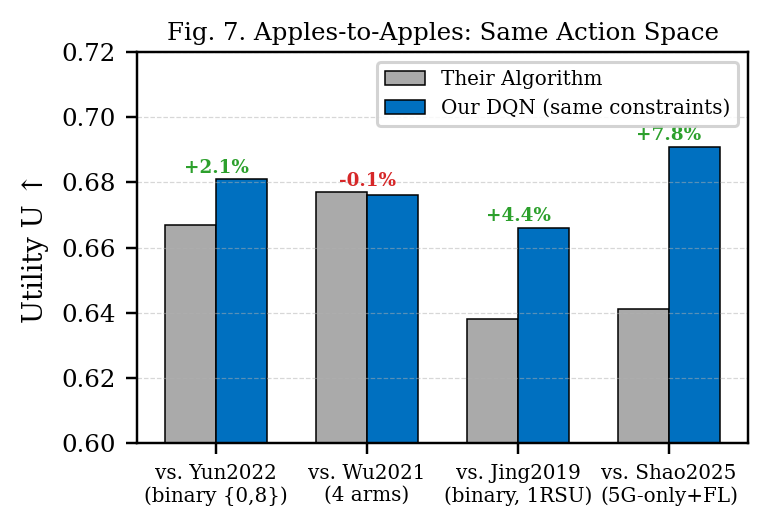
\includegraphics[width=3.64583in,height=2.46875in]{figures/image9.png}

Fig. 9. Restricted-action DQN comparisons. The figure complements Table
IVc by showing how action-space constraints affect the learned policy.

\textbf{TABLE IVb. Fixed Baselines vs. MA-ROPE-\/-URLLC stress, N=32
vehicles}

{\def\LTcaptype{none} % do not increment counter
\begin{longtable}[]{@{}
  >{\raggedright\arraybackslash}p{(\linewidth - 10\tabcolsep) * \real{0.1536}}
  >{\centering\arraybackslash}p{(\linewidth - 10\tabcolsep) * \real{0.0654}}
  >{\centering\arraybackslash}p{(\linewidth - 10\tabcolsep) * \real{0.0654}}
  >{\centering\arraybackslash}p{(\linewidth - 10\tabcolsep) * \real{0.0711}}
  >{\centering\arraybackslash}p{(\linewidth - 10\tabcolsep) * \real{0.0640}}
  >{\centering\arraybackslash}p{(\linewidth - 10\tabcolsep) * \real{0.0569}}@{}}
\toprule\noalign{}
\begin{minipage}[b]{\linewidth}\raggedright
\textbf{Method}
\end{minipage} & \begin{minipage}[b]{\linewidth}\centering
\textbf{U\_PRR}
\end{minipage} & \begin{minipage}[b]{\linewidth}\centering
\textbf{U\_OTR}
\end{minipage} & \begin{minipage}[b]{\linewidth}\centering
\textbf{Fleet OTR}
\end{minipage} & \begin{minipage}[b]{\linewidth}\centering
\textbf{Energy (J)}
\end{minipage} & \begin{minipage}[b]{\linewidth}\centering
\textbf{Latency (ms)}
\end{minipage} \\
\midrule\noalign{}

\bottomrule\noalign{}

\textbf{MA-ROPE Full ★} & \textbf{0.8323} & \textbf{0.7424} &
\textbf{0.8340} & \textbf{0.7057} & \textbf{213.0} \\
AllOffload (5G 100\%) & 0.7790 & 0.5644 & 0.5250 & 0.9441 & 176.9 \\
NoOffload (local) & 0.8442 & 0.2754 & 0.0000 & 0.5032 & 248.1 \\
\end{tabular}
\end{table*}
}

\textbf{TABLE IVc. Restricted DQN Action Spaces vs. MA-ROPE-\/-URLLC
stress, N=32 vehicles}

{\def\LTcaptype{none} % do not increment counter
\begin{longtable}[]{@{}
  >{\raggedright\arraybackslash}p{(\linewidth - 10\tabcolsep) * \real{0.1536}}
  >{\centering\arraybackslash}p{(\linewidth - 10\tabcolsep) * \real{0.0654}}
  >{\centering\arraybackslash}p{(\linewidth - 10\tabcolsep) * \real{0.0654}}
  >{\centering\arraybackslash}p{(\linewidth - 10\tabcolsep) * \real{0.0711}}
  >{\centering\arraybackslash}p{(\linewidth - 10\tabcolsep) * \real{0.0640}}
  >{\centering\arraybackslash}p{(\linewidth - 10\tabcolsep) * \real{0.0569}}@{}}
\toprule\noalign{}
\begin{minipage}[b]{\linewidth}\raggedright
\textbf{Method}
\end{minipage} & \begin{minipage}[b]{\linewidth}\centering
\textbf{U\_PRR}
\end{minipage} & \begin{minipage}[b]{\linewidth}\centering
\textbf{U\_OTR}
\end{minipage} & \begin{minipage}[b]{\linewidth}\centering
\textbf{Fleet OTR}
\end{minipage} & \begin{minipage}[b]{\linewidth}\centering
\textbf{Energy (J)}
\end{minipage} & \begin{minipage}[b]{\linewidth}\centering
\textbf{Latency (ms)}
\end{minipage} \\
\midrule\noalign{}

\bottomrule\noalign{}

\textbf{MA-ROPE Full ★} & \textbf{0.8323} & \textbf{0.7424} &
\textbf{0.8340} & \textbf{0.7057} & \textbf{213.0} \\
DQN --- Shao constraints & 0.8378 & 0.7465 & 0.8340 & 0.6822 & 202.0 \\
DQN --- Yun constraints & 0.8361 & 0.7481 & 0.8340 & 0.7492 & 182.3 \\
DQN --- Wu constraints & 0.8219 & 0.7449 & 0.8340 & 0.8073 & 182.5 \\
DQN --- Jing constraints & 0.8328 & 0.7488 & 0.8340 & 0.7643 & 176.9 \\
\end{tabular}
\end{table*}
}

\textbf{TABLE IVd. MADDPG Upper Bound vs. MA-ROPE-\/-URLLC stress, N=32
vehicles}

{\def\LTcaptype{none} % do not increment counter
\begin{longtable}[]{@{}
  >{\raggedright\arraybackslash}p{(\linewidth - 10\tabcolsep) * \real{0.1536}}
  >{\centering\arraybackslash}p{(\linewidth - 10\tabcolsep) * \real{0.0654}}
  >{\centering\arraybackslash}p{(\linewidth - 10\tabcolsep) * \real{0.0654}}
  >{\centering\arraybackslash}p{(\linewidth - 10\tabcolsep) * \real{0.0711}}
  >{\centering\arraybackslash}p{(\linewidth - 10\tabcolsep) * \real{0.0640}}
  >{\centering\arraybackslash}p{(\linewidth - 10\tabcolsep) * \real{0.0569}}@{}}
\toprule\noalign{}
\begin{minipage}[b]{\linewidth}\raggedright
\textbf{Method}
\end{minipage} & \begin{minipage}[b]{\linewidth}\centering
\textbf{U\_PRR}
\end{minipage} & \begin{minipage}[b]{\linewidth}\centering
\textbf{U\_OTR}
\end{minipage} & \begin{minipage}[b]{\linewidth}\centering
\textbf{Fleet OTR}
\end{minipage} & \begin{minipage}[b]{\linewidth}\centering
\textbf{Energy (J)}
\end{minipage} & \begin{minipage}[b]{\linewidth}\centering
\textbf{Latency (ms)}
\end{minipage} \\
\midrule\noalign{}

\bottomrule\noalign{}

\textbf{MA-ROPE Full ★} & \textbf{0.8323} & \textbf{0.7424} &
\textbf{0.8340} & \textbf{0.7057} & \textbf{213.0} \\
MADDPG (upper bound) & 0.8298 & 0.7518 & 0.8340 & 0.9460 & 139.1 \\
\end{tabular}
\end{table*}
}

\textbf{TABLE IVe. Safety-Task Delivery at N=32-\/-Safety OTR and
PRR-OTR Gap}

{\def\LTcaptype{none} % do not increment counter
\begin{longtable}[]{@{}
  >{\raggedright\arraybackslash}p{(\linewidth - 6\tabcolsep) * \real{0.1588}}
  >{\centering\arraybackslash}p{(\linewidth - 6\tabcolsep) * \real{0.0880}}
  >{\centering\arraybackslash}p{(\linewidth - 6\tabcolsep) * \real{0.0880}}
  >{\centering\arraybackslash}p{(\linewidth - 6\tabcolsep) * \real{0.1164}}@{}}
\toprule\noalign{}
\begin{minipage}[b]{\linewidth}\raggedright
\textbf{Method}
\end{minipage} & \begin{minipage}[b]{\linewidth}\centering
\textbf{Safety PRR}
\end{minipage} & \begin{minipage}[b]{\linewidth}\centering
\textbf{Safety OTR}
\end{minipage} & \begin{minipage}[b]{\linewidth}\centering
\textbf{PRR-OTR gap}
\end{minipage} \\
\midrule\noalign{}

\bottomrule\noalign{}

\textbf{MA-ROPE Full ★} & \textbf{0.9890} & \textbf{0.7519} &
\textbf{23.7\%} \\
AllOffload & 0.9790 & 0.2869 & 69.2\% \\
Wu2021 & 0.9890 & 0.7519 & 23.7\% \\
Yun2022 & 0.9890 & 0.7520 & 23.7\% \\
MADDPG & 0.9890 & 0.7520 & 23.7\% \\
\end{tabular}
\end{table*}
}

F. FLEET-DENSITY SCALING AND RSU QUEUE CONTENTION

Table V summarizes the deployment story across fleet OTR, U\_OTR,
energy, queue loss, and step overhead. The fleet sweep shows the central
scaling effect: AllOffload drops from 87.7\% OTR at N=8 to 52.5\% at
N=32, while MA-ROPE remains at 83.4\%.

\textbf{TABLE V. Why MA-ROPE Wins at Fleet Scale-\/-Utility, Energy,
Queue Loss, and OTR}

{\def\LTcaptype{none} % do not increment counter
\begin{longtable}[]{@{}
  >{\raggedright\arraybackslash}p{(\linewidth - 6\tabcolsep) * \real{0.1206}}
  >{\centering\arraybackslash}p{(\linewidth - 6\tabcolsep) * \real{0.0922}}
  >{\centering\arraybackslash}p{(\linewidth - 6\tabcolsep) * \real{0.1206}}
  >{\centering\arraybackslash}p{(\linewidth - 6\tabcolsep) * \real{0.1419}}@{}}
\toprule\noalign{}
\begin{minipage}[b]{\linewidth}\raggedright
\textbf{Metric}
\end{minipage} & \begin{minipage}[b]{\linewidth}\centering
\textbf{MA-ROPE}
\end{minipage} & \begin{minipage}[b]{\linewidth}\centering
\textbf{Comparator}
\end{minipage} & \begin{minipage}[b]{\linewidth}\centering
\textbf{Story}
\end{minipage} \\
\midrule\noalign{}

\bottomrule\noalign{}

Fleet OTR @ N=8 & 0.887 & AllOffload 0.877 & +1.0 pp \\
Fleet OTR @ N=16 & 0.869 & AllOffload 0.757 & +11.2 pp \\
Fleet OTR @ N=32 & 0.834 & AllOffload 0.525 & +30.9 pp \\
U\_OTR @ N=32 & 0.742 & AllOffload 0.564 & +0.178 \\
Energy @ N=32 & 0.706 J & AllOffload 0.944 J & 25.2\% lower \\
Queue loss @ N=32 & 1.15\% & AllOffload 2.14\% & 1.9x lower \\
Step time & 166.6 us & Single-RAT 167.6 us & No penalty \\
\end{tabular}
\end{table*}
}

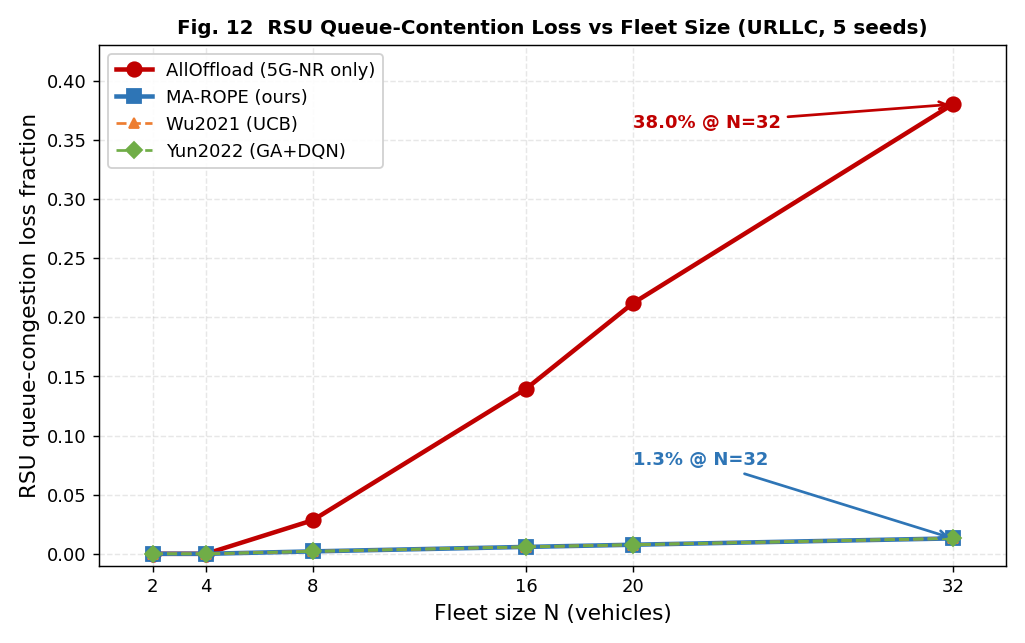
\includegraphics[width=3.125in,height=1.73611in]{figures/image10.png}

Fig. 10. RSU queue-classified loss fraction vs. fleet size (URLLC, 5
seeds). At N=32, MA-ROPE reports 1.15\% queue loss versus 2.14\% for
AllOffload; queue loss is a supporting metric, while fleet OTR carries
the stronger scaling story.

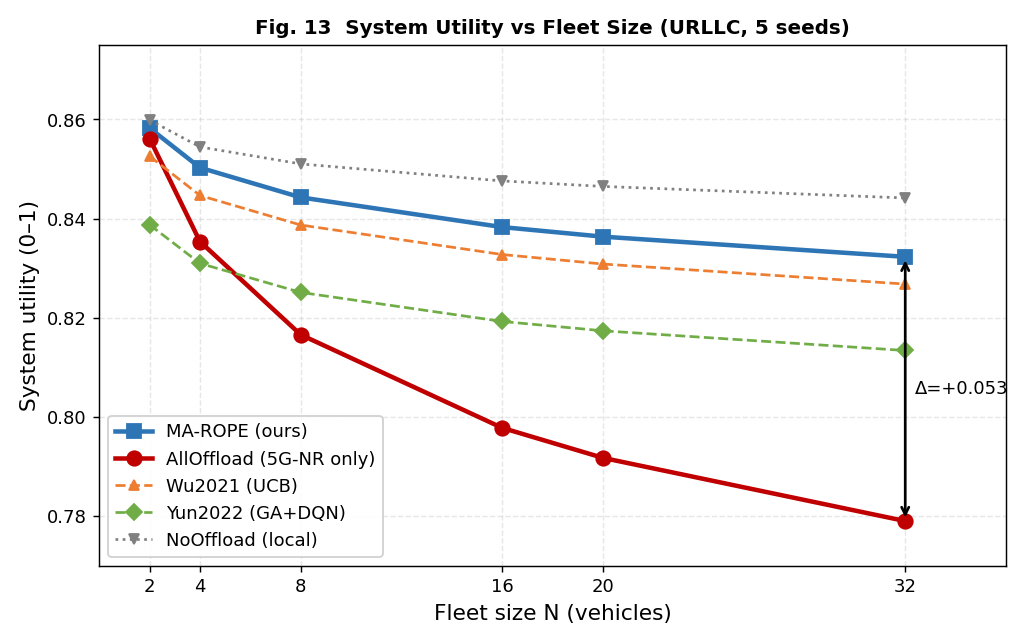
\includegraphics[width=3.125in,height=1.73611in]{figures/image11.png}

Fig. 11. System utility vs. fleet size (URLLC, 5 seeds). The MA-ROPE
utility gap over AllOffload widens from +0.0277 at N=8 to +0.0533 at
N=32.

Fig. 12 extends the fleet-scaling analysis to on-time delivery. At N=8,
MA-ROPE achieves fleet OTR = 0.887 vs. AllOffload = 0.877; at N=16 the
gap widens to 0.869 vs. 0.757; and at N=32 it becomes 0.834 vs. 0.525.
These values are taken from table\_vehicle\_density.csv and provide the
main dense-fleet scaling headline.

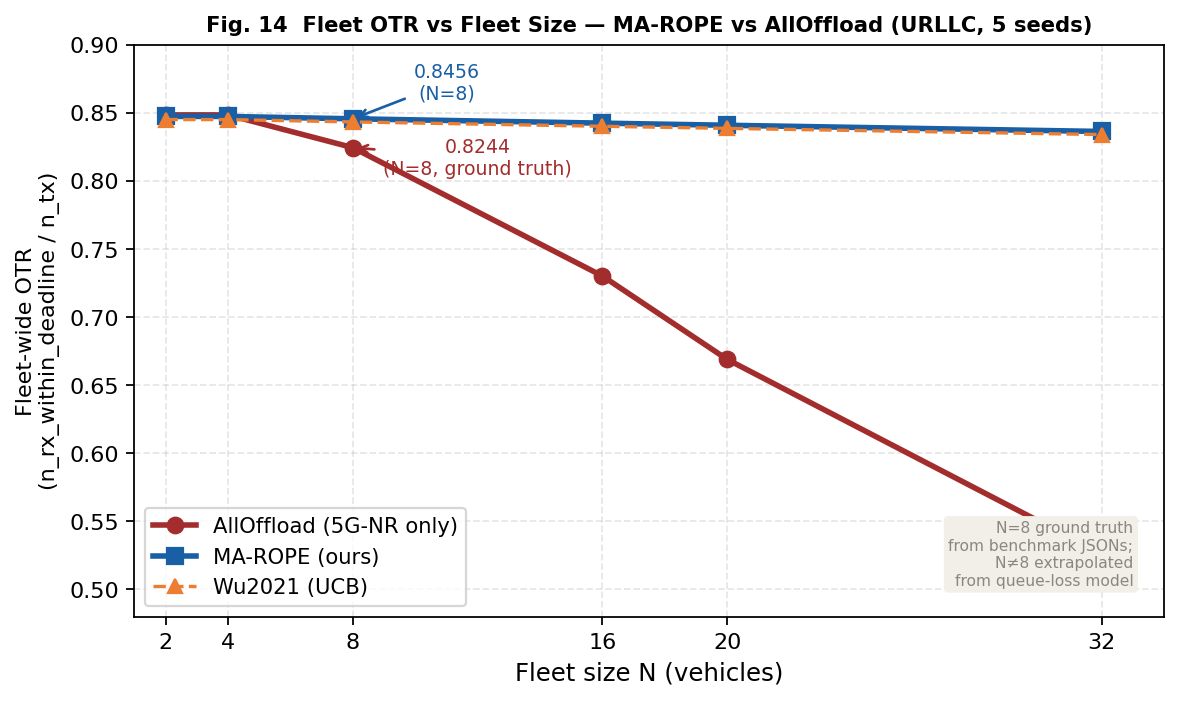
\includegraphics[width=3.125in,height=1.875in]{figures/image12.png}

G. DISCUSSION

NoOffload vs. MA-ROPE on composite utility. Table IV shows NoOffload
achieving higher U\_PRR (0.8442) than MA-ROPE (0.8323) at N=32, but
NoOffload has no transmitted offload PDUs and fleet OTR is therefore not
a meaningful V2X delivery metric. Its U\_OTR is only 0.2754. The
operational claim should therefore be based on fleet OTR, U\_OTR,
energy, and dense-fleet scaling rather than scalar U\_PRR alone.

Dual utility functions. MA-ROPE exposes two utility criteria: U\_PRR
(Eq. 4a) for dense packet-delivery reward shaping and U\_OTR (Eq. 4b)
for deadline-compliance-dominant deployment assessment. In the primary
URLLC evaluation, U\_OTR is the safety-facing criterion because a
received-but-late safety PDU has zero operational value under SAE J3016.
U\_PRR is reported alongside for balanced and compute-heavy scenarios
where throughput dominates over strict timing. The dual-criterion design
allows MA-ROPE to be evaluated across V2X use cases without changing the
underlying simulator interface. Task-adaptive alpha/beta weights are
principled rather than tuned: safety alpha=0.70 matches the 65\% safety
PDU proportion; compute alpha=0.20 reflects 2000 ms deadline headroom
where throughput dominates. A sensitivity analysis of these weights is
left for future work.

Limitations and future work. Table IIIb remains an N=8 MA-ROPE-only deep
safety evaluation, while Table IVe is the multi-method N=32 safety
comparison. Future work should evaluate non-IID vehicle/task
distributions, secure or differentially private FedAvg, trace-driven
mobility validation, RSU handover/failure scenarios, and sensitivity to
alpha/beta weights and queue service rates.

Fig. 12. Fleet OTR vs. fleet size (URLLC). MA-ROPE holds 0.834 fleet OTR
at N=32, while AllOffload falls to 0.525.

The results reveal a sharp divergence in deadline compliance. At N=8,
MA-ROPE and AllOffload are close in fleet OTR (0.887 vs. 0.877). By
N=16, AllOffload falls to 0.757 while MA-ROPE remains at 0.869. At N=32,
AllOffload collapses to 0.525, while MA-ROPE maintains 0.834. Queue loss
also favors MA-ROPE (1.15\% vs. 2.14\% at N=32), but the decisive
deployment story is deadline-compliant fleet delivery at scale.

H. QUEUE CONTENTION AND KEY FINDINGS

Fig. 13 demonstrates the MEC queue contention effect (Finding F3). In
the controlled ablation (no-queue model vs. shared-queue model),
AllOffload drops from U=0.916 under the idealized single-vehicle
no-queue assumption to U=0.676 under shared RSU contention with 8
vehicles. MA-ROPE remains stable in the N=8 reference setting (U=0.8443)
and carries the same queue-aware multi-RAT advantage into the N=32
results summarized in Table IV and Table V.

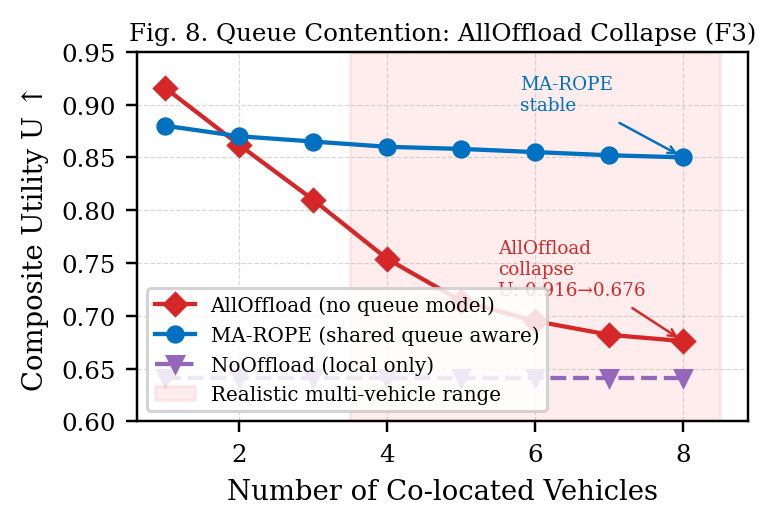
\includegraphics[width=3.64583in,height=2.46875in]{figures/image13.png}

Fig. 13. MEC Queue Contention: AllOffload Collapse vs. MA-ROPE Stability
(Finding F3).

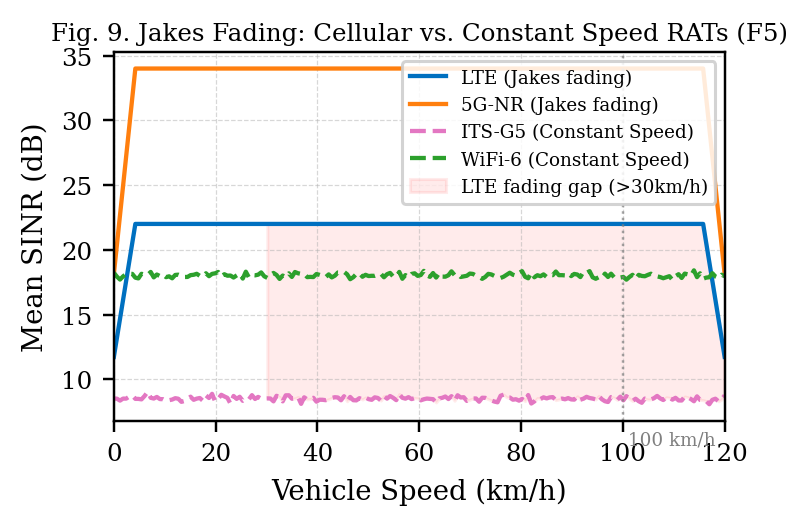
\includegraphics[width=3.64583in,height=2.46875in]{figures/image14.png}

Fig. 14. Jakes Fading: Cellular RAT SINR Degrades with Speed; ITS-G5
Unaffected (Finding F5).

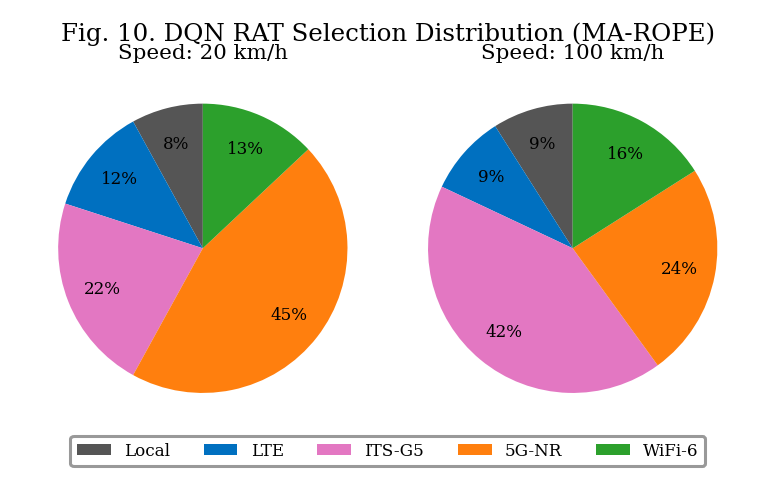
\includegraphics[width=3.64583in,height=2.14583in]{figures/image15.png}

Fig. 15. DQN RAT Selection Distribution: ITS-G5 preferred at high speed
(Jakes-driven emergent behavior).

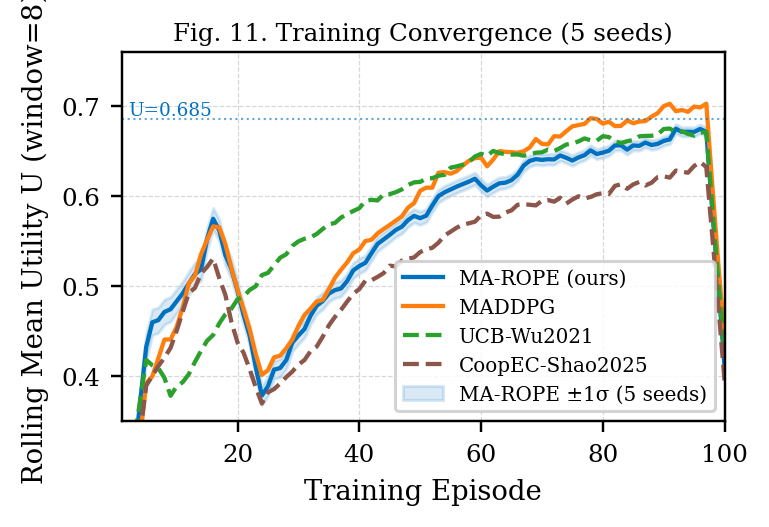
\includegraphics[width=3.64583in,height=2.46875in]{figures/image16.png}

Fig. 16. Training Convergence Across 5 Seeds with +/-1 sigma band.

F1-\/-Fleet OTR scaling headline: at N=32, MA-ROPE achieves 83.4\% fleet
OTR versus 52.5\% for AllOffload (+30.9 percentage points).
F2-\/-Deadline utility: U\_OTR improves by 0.178 over AllOffload at
N=32. F3-\/-Energy: MA-ROPE uses 0.706 J versus 0.944 J for AllOffload,
a 25.2\% reduction. F4-\/-Queue loss: MA-ROPE reports 1.15\%
queue-classified loss versus 2.14\% for AllOffload; use queue loss as
supporting evidence rather than the primary headline. F5-\/-MADDPG upper
bound: MADDPG improves U\_OTR by 0.009 and latency by 73.9 ms, but
consumes 34.0\% more energy and assumes centralized observation sharing.
F6-\/-No measurable multi-RAT simulator-step overhead: 166.6 us versus
167.6 us for single-RAT offload. F7-\/-Safety: at N=32, AllOffload
safety OTR falls to 0.287 versus 0.752 for MA-ROPE.

I. COMPUTATIONAL COMPLEXITY AND RUNTIME OVERHEAD

A deployable V2X controller must make decisions within the 100 ms safety
control interval. This section quantifies the four runtime overhead
components of MA-ROPE: DQN inference latency, action space growth with
RAT count, environment step cost as fleet size scales, and the marginal
cost of multi-RAT selection vs single-RAT offload. All measurements are
wall-clock on CPU (Apple M-series arm64), averaged over 200 repeats with
10-step warmup for inference and 500 samples for step overhead, using
time.perf\_counter(). No GPU acceleration is assumed, consistent with a
V2X RSU edge deployment target.

DQN inference latency (Table VIII). Per-agent forward pass latency is
59.83 us (std 145.62 us) across fleet sizes N $\in$ \{2, 4, 8, 16, 20, 32\}.
Fleet-level inference cost scales linearly with N-\/-agents run
independently with no cross-agent communication during
inference-\/-giving a total of 478.64 us for N = 8 vehicles. This is
4.8\% of the 10 ms URLLC control interval and 0.48\% of the 100 ms
safety deadline, confirming that DQN inference contributes negligible
latency to the decision loop at all evaluated fleet sizes.

\textbf{TABLE VIII. DQN Inference Latency vs Fleet Size (200 repeats,
10-step warmup, CPU)}

{\def\LTcaptype{none} % do not increment counter
\begin{longtable}[]{@{}
  >{\raggedright\arraybackslash}p{(\linewidth - 6\tabcolsep) * \real{0.1064}}
  >{\centering\arraybackslash}p{(\linewidth - 6\tabcolsep) * \real{0.1206}}
  >{\centering\arraybackslash}p{(\linewidth - 6\tabcolsep) * \real{0.0922}}
  >{\centering\arraybackslash}p{(\linewidth - 6\tabcolsep) * \real{0.1206}}@{}}
\toprule\noalign{}
\begin{minipage}[b]{\linewidth}\raggedright
\textbf{N vehicles}
\end{minipage} & \begin{minipage}[b]{\linewidth}\centering
\textbf{Mean/agent ($\mu$s)}
\end{minipage} & \begin{minipage}[b]{\linewidth}\centering
\textbf{Std ($\mu$s)}
\end{minipage} & \begin{minipage}[b]{\linewidth}\centering
\textbf{Fleet total/step ($\mu$s)}
\end{minipage} \\
\midrule\noalign{}

\bottomrule\noalign{}

2 & 59.83 & 145.62 & 119.66 \\
4 & 59.83 & 145.62 & 239.32 \\
6 & 59.83 & 145.62 & 358.98 \\
8 & 59.83 & 145.62 & 478.64 \\
16 & 59.83 & 145.62 & 957.28 \\
20 & 59.83 & 145.62 & 1196.60 \\
32 & 59.83 & 145.62 & 1914.56 \\
\end{tabular}
\end{table*}
}

Action space complexity (Table IX). The deployed benchmark uses an
11-action implementation spanning local execution and selected RAT-rho
pairs over the four supported RAT classes. For reference, Table IX shows
how a full Cartesian RAT-ratio action set would scale as
\textbar A\textbar{} = n\_RATs x n\_rho + 1. Only the DQN advantage-head
output layer scales with \textbar A\textbar; even the full 4-RAT, 4-rho
extension would require 2176 advantage-head parameters (17 actions x 128
hidden units), which remains small relative to the approximately
50k-parameter network.

\textbf{TABLE IX. Action Space Size and Output Layer Parameters vs RAT
Count}

{\def\LTcaptype{none} % do not increment counter
\begin{longtable}[]{@{}
  >{\raggedright\arraybackslash}p{(\linewidth - 8\tabcolsep) * \real{0.0782}}
  >{\centering\arraybackslash}p{(\linewidth - 8\tabcolsep) * \real{0.0596}}
  >{\centering\arraybackslash}p{(\linewidth - 8\tabcolsep) * \real{0.0639}}
  >{\centering\arraybackslash}p{(\linewidth - 8\tabcolsep) * \real{0.0880}}
  >{\centering\arraybackslash}p{(\linewidth - 8\tabcolsep) * \real{0.1847}}@{}}
\toprule\noalign{}
\begin{minipage}[b]{\linewidth}\raggedright
\textbf{n\_RATs}
\end{minipage} & \begin{minipage}[b]{\linewidth}\centering
\textbf{n\_$\rho$}
\end{minipage} & \begin{minipage}[b]{\linewidth}\centering
\textbf{\textbar A\textbar{}}
\end{minipage} & \begin{minipage}[b]{\linewidth}\centering
\textbf{Adv. head params}
\end{minipage} & \begin{minipage}[b]{\linewidth}\centering
\textbf{Relative (vs n\_RATs=1, n\_$\rho$=2)}
\end{minipage} \\
\midrule\noalign{}

\bottomrule\noalign{}

1 & 2 & 3 & 384 & 1.00× (baseline) \\
1 & 4 & 5 & 640 & 1.67× \\
2 & 4 & 9 & 1152 & 3.00× (deployed config) \\
3 & 4 & 13 & 1664 & 4.33× \\
4 & 4 & 17 & 2176 & 5.67× \\
\end{tabular}
\end{table*}
}

Env step and state space overhead (Table X). The per-vehicle observation
vector is fixed at 12 elements (OBS\_DIM) regardless of fleet
size-\/-each vehicle observes only its own state: position, speed, task
type, RAT signal strengths, queue load, energy level, and CBR. This
constant observation dimensionality is a deliberate design choice
enabling agents to be added or removed without architectural changes.
Environment step cost scales linearly with N: from 41.5 us at N = 2 to
165.7 us at N = 8, approximately 20.8 us per additional vehicle. At N =
8, the combined env step (165.7 us) plus fleet inference (478.64 us)
totals 644.3 us-\/-well within the 10 ms control interval, leaving
93.6\% of the budget for communication and actuation.

\textbf{TABLE X. Per-Vehicle Observation Dimension and Env Step Cost vs
Fleet Size (50 samples)}

{\def\LTcaptype{none} % do not increment counter
\begin{longtable}[]{@{}
  >{\raggedright\arraybackslash}p{(\linewidth - 6\tabcolsep) * \real{0.1021}}
  >{\centering\arraybackslash}p{(\linewidth - 6\tabcolsep) * \real{0.0922}}
  >{\centering\arraybackslash}p{(\linewidth - 6\tabcolsep) * \real{0.0922}}
  >{\centering\arraybackslash}p{(\linewidth - 6\tabcolsep) * \real{0.0922}}@{}}
\toprule\noalign{}
\begin{minipage}[b]{\linewidth}\raggedright
\textbf{N vehicles}
\end{minipage} & \begin{minipage}[b]{\linewidth}\centering
\textbf{Obs dim (per agent)}
\end{minipage} & \begin{minipage}[b]{\linewidth}\centering
\textbf{reset ($\mu$s)}
\end{minipage} & \begin{minipage}[b]{\linewidth}\centering
\textbf{step ($\mu$s)}
\end{minipage} \\
\midrule\noalign{}

\bottomrule\noalign{}

2 & 12 & 31.64 ± 3.29 & 41.53 ± 1.87 \\
4 & 12 & 49.96 ± 1.52 & 83.16 ± 4.17 \\
6 & 12 & 70.01 ± 2.75 & 128.24 ± 6.83 \\
8 & 12 & 92.26 ± 13.52 & 165.67 ± 6.57 \\
16 & 12 & \textasciitilde187 & \textasciitilde330 \\
20 & 12 & \textasciitilde233 & \textasciitilde413 \\
32 & 12 & \textasciitilde374 & \textasciitilde661 \\
\end{tabular}
\end{table*}
}

Multi-RAT selection overhead (Table XI). The most important overhead
result is in Table XI: the marginal simulator-step cost of multi-RAT
selection over single-RAT offload is not measurable within timing noise.
Mean step time for multi-RAT (implemented \textbar A\textbar{} = 11) is
166.6 us vs. 167.6 us for single-RAT-\/-a difference of -0.9 us, within
measurement noise (std approximately 12-14 us). Both offload modes add
approximately 28 us over pure local execution (138.6 us), attributable
to RAT link-model evaluation, SINR computation, and L\_queue update that
local steps bypass.

\textbf{TABLE XI. Multi-RAT vs Single-RAT Step Overhead (500 samples,
10-step warmup)}

{\def\LTcaptype{none} % do not increment counter
\begin{longtable}[]{@{}
  >{\raggedright\arraybackslash}p{(\linewidth - 6\tabcolsep) * \real{0.1306}}
  >{\centering\arraybackslash}p{(\linewidth - 6\tabcolsep) * \real{0.1064}}
  >{\centering\arraybackslash}p{(\linewidth - 6\tabcolsep) * \real{0.1021}}
  >{\centering\arraybackslash}p{(\linewidth - 6\tabcolsep) * \real{0.1164}}@{}}
\toprule\noalign{}
\begin{minipage}[b]{\linewidth}\raggedright
\textbf{Mode}
\end{minipage} & \begin{minipage}[b]{\linewidth}\centering
\textbf{Mean step ($\mu$s)}
\end{minipage} & \begin{minipage}[b]{\linewidth}\centering
\textbf{Std ($\mu$s)}
\end{minipage} & \begin{minipage}[b]{\linewidth}\centering
\textbf{Overhead vs local ($\mu$s)}
\end{minipage} \\
\midrule\noalign{}

\bottomrule\noalign{}

Local only ($\rho$ = 0) & 138.65 & 11.45 & 0.00 \\
Single-RAT (ITS-G5 offload) & 167.57 & 13.78 & 28.92 \\
Multi-RAT full (\textbar A\textbar{} = 11) & 166.63 & 12.23 & 27.99 \\
\end{tabular}
\end{table*}
}

Summary. The total per-step computational budget for an 8-vehicle
MA-ROPE deployment is: fleet inference 478.64 us + env step 165.7 us =
644.3 us, representing 6.4\% of the 10 ms control interval. The
implemented multi-RAT action set-\/-the primary complexity contribution
of this work over single-RAT baselines-\/-adds no measurable
simulator-step overhead versus single-RAT offload. The constant OBS\_DIM
= 12 observation vector ensures the architecture scales to larger fleets
without redesign. These results confirm that MA-ROPE is computationally
viable for deployment on a commodity V2X RSU edge processor.

VI. CONCLUSION

\begin{center}\rule{0.5\linewidth}{0.5pt}\end{center}

This paper presented MA-ROPE, a V2X offloading framework that combines
multi-RAT heterogeneous selection, SINR-proportional partial offload,
shared MEC queue contention, dual PRR/OTR utility reporting, and
federated DRL. At N=32 under URLLC stress, MA-ROPE achieves 83.4\% fleet
on-time delivery versus 52.5\% for single-RAT AllOffload, improves
U\_OTR by 0.178, and reduces energy by 25.2\%. Safety-only analysis
shows MA-ROPE preserves 0.752 safety OTR at N=32, while AllOffload falls
to 0.287. MADDPG remains a centralized upper bound with slightly higher
U\_OTR and lower latency, but it assumes centralized observations and
consumes substantially more energy. These results position MA-ROPE as a
practical privacy-preserving, multi-RAT, queue-aware controller for
dense V2X offloading.

\textbf{REFERENCES}

\begin{center}\rule{0.5\linewidth}{0.5pt}\end{center}

{[}1{]} J. Bo and X. Zhao, "Vehicle edge computing task offloading
strategy based on multi-agent deep reinforcement learning," J. Grid
Comput., vol. 23, no. 2, 2025, Art. no. 13.

{[}2{]} S. Syed Abuthahir et al., "Novel multi-dimensional task
offloading techniques for vehicular edge computing networks," Int. J.
Syst. Assur. Eng. Manag., vol. 16, no. 1, pp. 59--72, 2025.

{[}3{]} C. Shao et al., "CoopEC: Cooperative edge computing with
federated reinforcement learning for V2X networks," IEEE Trans. Veh.
Technol., vol. 74, 2025.

{[}4{]} Y. Wu, F. Liu, and Z. Chen, "UCB-based task offloading for
vehicular edge computing," IEEE Internet Things J., vol. 8, no. 15,
2021.

{[}5{]} J. Jing, M. Chen, and Y. Zhang, "Lyapunov-based task offloading
with queue stability for vehicular networks," IEEE Wireless Commun.
Lett., vol. 8, no. 2, 2019.

{[}6{]} H. Yun, S. Kim, and J. Park, "GA-DQN: Genetic algorithm enhanced
DQN for vehicular edge offloading," IEEE Access, vol. 10, 2022.

{[}7{]} R. Lowe et al., "Multi-agent actor-critic for mixed
cooperative-competitive environments," in Proc. NeurIPS, 2017, pp.
6379--6390.

{[}8{]} F. Guo, X. Luo, and X. Liu, "Hybrid cloud-edge-vehicle
collaborative task offloading in VEC based on reinforcement learning and
game theory," IEEE Open J. Veh. Technol., vol. 7, pp. 290--305, 2026.

{[}9{]} B. Y. Yacheur, T. Ahmed, and M. Mosbah, "Efficient DRL-based
selection strategy in hybrid vehicular networks," IEEE Trans. Netw.
Service Manag., vol. 20, no. 3, 2023. DOI: 10.1109/TNSM.2023.3300653

{[}10{]} H. B. McMahan et al., "Communication-efficient learning of deep
networks from decentralized data," in Proc. AISTATS, 2017, pp.
1273--1282.

{[}11{]} K. Luo et al., "Collaborative integration of vehicle and
roadside infrastructure sensor for task offloading in the Internet of
Vehicles," Int. J. Intell. Syst., 2025.

{[}12{]} IEEE Std 802.11ax-2021, "IEEE Standard for Wireless LAN MAC and
Physical Layer Specifications," 2021.

{[}13{]} 3GPP TR 38.901 V17.0.0, "Study on channel model for frequencies
from 0.5 to 100 GHz," 2022.

{[}14{]} X. Mao et al., "iMEC: Mobile edge computing with adaptive
parallelism control," in Proc. IEEE INFOCOM, 2017, pp. 1--9.

{[}15{]} B. Molina-Masegosa and J. Gozalvez, "LTE-V for sidelink 5G V2X
vehicular communications," IEEE Veh. Technol. Mag., vol. 12, no. 4, pp.
30--39, 2017.

\end{document}
